%%%%%%%%%%%%%%%%%%%%%%%%%%%%%%%%%%%%%%%%%
% Beamer Presentation
% LaTeX Template
% Version 1.0 (10/11/12)
%
% This template has been downloaded from:
% http://www.LaTeXTemplates.com
%
% License:
% CC BY-NC-SA 3.0 (http://creativecommons.org/licenses/by-nc-sa/3.0/)
%
%%%%%%%%%%%%%%%%%%%%%%%%%%%%%%%%%%%%%%%%%

%----------------------------------------------------------------------------------------
%	PACKAGES AND THEMES
%----------------------------------------------------------------------------------------

\documentclass{beamer}

\mode<presentation> {

% The Beamer class comes with a number of default slide themes
% which change the colors and layouts of slides. Below this is a list
% of all the themes, uncomment each in turn to see what they look like.

%\usetheme{default}
%\usetheme{AnnArbor}
%\usetheme{Antibes}
%\usetheme{Bergen}
% \usetheme{Berkeley}
%\usetheme{Berlin}
%\usetheme{Boadilla}
% \usetheme{CambridgeUS}
% \usetheme{Copenhagen}
%\usetheme{Darmstadt}
%\usetheme{Dresden}
\usetheme{Frankfurt}
% \usetheme{Goettingen}
% \usetheme{Hannover}
% \usetheme{Ilmenau}
%\usetheme{JuanLesPins}
%\usetheme{Luebeck}
%\usetheme{Madrid}
%\usetheme{Malmoe}
%\usetheme{Marburg}
%\usetheme{Montpellier}
%\usetheme{PaloAlto}
% \usetheme{Pittsburgh}
%\usetheme{Rochester}
%\usetheme{Singapore}
%\usetheme{Szeged}
%\usetheme{Warsaw}

% As well as themes, the Beamer class has a number of color themes
% for any slide theme. Uncomment each of these in turn to see how it
% changes the colors of your current slide theme.

%\usecolortheme{albatross}
%\usecolortheme{beaver}
%\usecolortheme{beetle}
%\usecolortheme{crane}
%\usecolortheme{dolphin}
%\usecolortheme{dove}
%\usecolortheme{fly}
%\usecolortheme{lily}
%\usecolortheme{orchid}
%\usecolortheme{rose}
%\usecolortheme{seagull}
%\usecolortheme{seahorse}
%\usecolortheme{whale}
%\usecolortheme{wolverine}

%\setbeamertemplate{footline} % To remove the footer line in all slides uncomment this line
%\setbeamertemplate{footline}[page number] % To replace the footer line in all slides with a simple slide count uncomment this line

%\setbeamertemplate{navigation symbols}{} % To remove the navigation symbols from the bottom of all slides uncomment this line
}

\usepackage{graphicx} % Allows including images
\usepackage{booktabs} % Allows the use of \toprule, \midrule and \bottomrule in tables

% Format citation
\usepackage[backend=biber,style=apa,citestyle=authoryear]{biblatex}
\DeclareLanguageMapping{bahasa}{american-apa}
\DeclareFieldFormat{apacase}{#1}
\bibliography{../src/references}

%----------------------------------------------------------------------------------------
%	TITLE PAGE
%----------------------------------------------------------------------------------------

\title[]{Pengembangan Pencocokan Paket Berbasis GPU pada Snort NIDS} % The short title appears at the bottom of every slide, the full title is only on the title page

\author{Afrizal Fikri - 13513004} % Your name
% 13513004
% \institute[UCLA] % Your institution as it will appear on the bottom of every slide, may be shorthand to save space
% {
% University of California \\ % Your institution for the title page
% \medskip
% \textit{john@smith.com} % Your email address
% }
% \date{\today} % Date, can be changed to a custom date

\begin{document}

\begin{frame}
\titlepage % Print the title page as the first slide
\end{frame}

\begin{frame}
\frametitle{Overview} % Table of contents slide, comment this block out to remove it
\tableofcontents % Throughout your presentation, if you choose to use \section{} and \subsection{} commands, these will automatically be printed on this slide as an overview of your presentation
\end{frame}

%----------------------------------------------------------------------------------------
%	PRESENTATION SLIDES
%----------------------------------------------------------------------------------------

%------------------------------------------------
\section{Latar Belakang} % Sections can be created in order to organize your presentation into discrete blocks, all sections and subsections are automatically printed in the table of contents as an overview of the talk
%------------------------------------------------

  \begin{frame}
  \frametitle{Intrusi Jaringan}
  \begin{itemize}
    \item Segala bentuk percobaan akses yang tidak berhak dalam suatu \emph{request} dalam jaringan
    \item Memiliki pola tertentu dalam 
    \item Contoh:
      \begin{itemize}
        \item \emph{Denial of Service} (DoS)
        \item \emph{Masquerading} (\emph{eavesdropping}, \emph{hijacking}, dll)
        \item \emph{Malware} (\emph{trojan}, \emph{virus}, \emph{worm}, dll)
      \end{itemize}
  \end{itemize}
  \end{frame}

  %------------------------------------------------

  \begin{frame}
  \frametitle{Intrusi Jaringan - \emph{Network Intrusion Detection System}}
  \begin{itemize}
    \item Sebuah sistem yang melakukan deteksi pola serangan
    \item Paket tidak diteruskan oleh NIDS (hanya disalin)
    \item Paket berbahaya hanya akan ditulis ke log atau juga dilaporkan ke admin
  \end{itemize}
  \end{frame}
  
  %------------------------------------------------

  \begin{frame}
  \frametitle{Intrusi Jaringan - \emph{Network Intrusion Detection System}}
  Ada 3 pendekatan NIDS:
  \begin{itemize}
    \item \emph{Signature-based} NIDS
    \item \emph{Anomaly-based} NIDS
    \item \emph{Stateful Protocol Analysis} NIDS
  \end{itemize}
  \end{frame}
  
  %------------------------------------------------

  \begin{frame}
  \frametitle{Intrusi Jaringan - \emph{Signature-based NIDS}}
  Ada 3 pendekatan NIDS:
  \begin{itemize}
    \item \emph{Signature-based NIDS}
    \item \emph{Anomaly-based NIDS}
    \item \emph{Stateful Protocol Analysis NIDS}
  \end{itemize}
  \end{frame}

  %------------------------------------------------

  \begin{frame}
  \frametitle{\emph{Network Intrusion Prevention System}}
  \begin{itemize}
    \item NIDS yang secara aktif mencegah kemungkinan serangan
    \item Paket harus melewati NIPS sebelum dapat melakukan akses ke sistem (\emph{blocking})
    \item Paket berbahaya akan ditolak
    \item Dapat memblok akses dari sumber yang sering terdeteksi mengandung paket berbahaya
    \item Kecepatan analisis sangat penting
  \end{itemize}
  \end{frame}

  %------------------------------------------------

  \begin{frame}
  \frametitle{Snort}
  \begin{columns}[c]
    \column{.45\textwidth}
    \begin{itemize}
      \item \emph{Signature-based} NIDS yang bersifat \emph{open-source}
      \item Bekerja dengan menggunakan \emph{rule} yang didefinisikan pengguna
      \item Memiliki 3 modus:
      \begin{itemize}
        \item Modus pengendus
        \item Modus pencatat
        \item Modus deteksi intrusi
      \end{itemize}
    \end{itemize}

    \column{.5\textwidth}
    \begin{figure}
      
\includegraphics[width=0.8\linewidth]{resources/snort.jpg}
    \end{figure}
  \end{columns}
  \end{frame}

  %------------------------------------------------

  \begin{frame}
  \frametitle{Snort - Komponen}
  \begin{itemize}
    \item Modul Penangkap Paket
    \item Modul \emph{Decoder}
    \item Modul Preproses
    \item Modul Detektor
    \item Modul Keluaran
  \end{itemize}
  \end{frame}

  %------------------------------------------------

  \begin{frame}
  \frametitle{Snort - \emph{Rule}}
  \emph{Rule} terdiri dari 2 bagian utama; \emph{header} dan \emph{option}
  \begin{figure}
    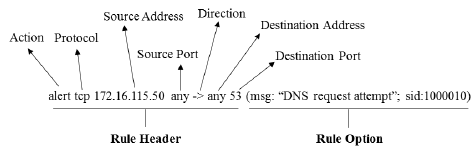
\includegraphics[width=0.8\linewidth]{../src/resources/rule.png}
  \end{figure}
  \end{frame}

  %------------------------------------------------

  \begin{frame}
  \frametitle{Pencocokan String}
  \begin{itemize}
    \item Metode mencari kemunculan sebuah string dalam string lain
    \item Dapat digunakan untuk mencari pola dalam \emph{payload} paket
    \item Ada 2 pendekatan berdasarkan jumlah yang string dicocokkan:
      \begin{itemize}
        \item \emph{Single pattern matching}
        \item \emph{Multi-pattern matching}
      \end{itemize}
  \end{itemize}
  \end{frame}

  %------------------------------------------------

  \begin{frame}
  \frametitle{Pencocokan String - Algoritma Aho-Corasick}
  \begin{itemize}
    \item Algoritma pencocokan string berbasis \emph{multi-pattern}
    \item Menggunakan \emph{finite automata} untuk mencocokkan string terhadap sebuah kumpulan string (kamus)
    \item Mengurangi jumlah \emph{backtrack} dengan \emph{failure function}
  \end{itemize}
  \end{frame}
  
  %------------------------------------------------

  \begin{frame}
  \frametitle{Pencocokan String - Algoritma Aho-Corasick}
  \begin{figure}
    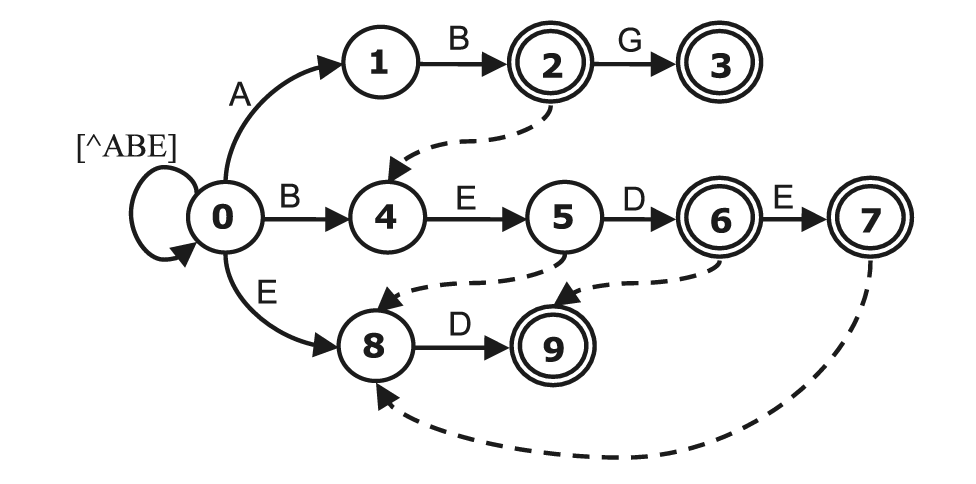
\includegraphics[width=0.8\linewidth]{../src/resources/aho-c.png}
  \end{figure}
  \end{frame}
  
  %------------------------------------------------

  \begin{frame}
  \frametitle{Pencocokan String - \emph{Multithread Aho-Corasick}}
  \begin{itemize}
    \item Tidak mudah melakukan partisi pada \emph{finite automata}
    \item \emph{Failure function} yang menjadi kelebihan algoritma ini pada \emph{single thread} malah menghambat pada desain \emph{multithread}
  \end{itemize}
  \end{frame}

  %------------------------------------------------

  \begin{frame}
  \frametitle{Pencocokan String - \emph{Parallel Failureless Aho-Corasick}}
  Sebagai solusi terhadap masalah partisi algoritma Aho-Corasick:
  \begin{itemize}
    \item Meminimalkan sinkronisasi antar \emph{thread}
    \item Masing-masing \emph{thread} mencocokkan satu pola
    \item Bagian otomata yang diakses tiap \emph{thread} saling independen
  \end{itemize}
  \end{frame}

  %------------------------------------------------

  \begin{frame}
  \frametitle{Pencocokan String - \emph{Parallel Failureless Aho-Corasick}}
  \begin{figure}
    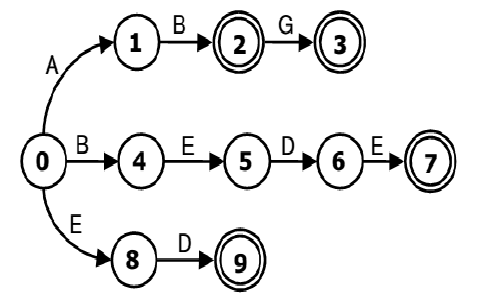
\includegraphics[width=0.8\linewidth]{../src/resources/pfac.png}
  \end{figure}
  \end{frame}

  %------------------------------------------------

  \begin{frame}
  \frametitle{\emph{Compute Unified Device Architecture}}
  \begin{itemize}
    \item Platform untuk komputasi non-grafik pada GPU (GPGPU)
    \item Cocok untuk melakukan operasi paralel dengan banyak \emph{thread}
    \item Mudah digunakan
    \item Hanya tersedia pada GPU NVIDIA
  \end{itemize}
  \end{frame}

  %------------------------------------------------

  \begin{frame}
  \frametitle{\emph{Compute Unified Device Architecture} - Organisasi \emph{Thread}}
  \begin{figure}
    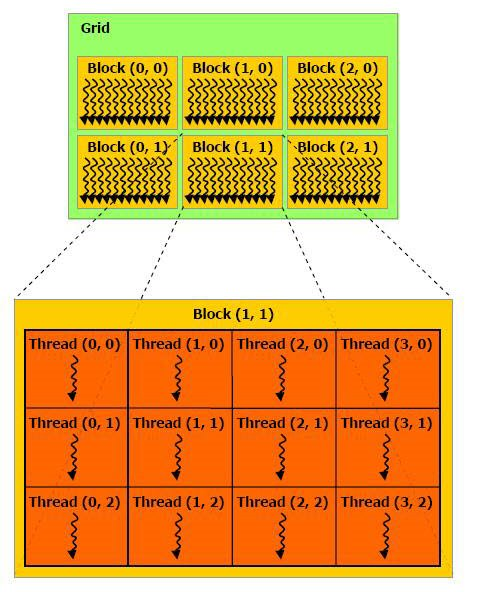
\includegraphics[width=0.5\linewidth]{../src/resources/cudathread.jpg}
  \end{figure}
  \end{frame}

  %------------------------------------------------

  \begin{frame}
  \frametitle{\emph{Compute Unified Device Architecture} - Organisasi Memori}
  Struktur memori:
  \begin{itemize}
    \item Memori lokal
    \item \emph{Shared memory}
    \item Memori global
  \end{itemize}

  Semakin besar lingkup memori, semakin lambat kecepatan akses
  \end{frame}

%------------------------------------------------
\section{Penelitian Terkait}
%------------------------------------------------

  % \subsection{Subsection Example} % A subsection can be created just before a set of slides with a common theme to further break down your presentation into chunks

  \begin{frame}
  \frametitle{Rancangan \emph{Multithreading} pada Pencocokan NIDS Berbasis \emph{Signature}}
  Berdasarkan penelitian oleh \cite{multi2004}:
  \begin{itemize}
    \item Rancangan yang diajukan:
    \begin{itemize}
      \item \emph{Thread} untuk modul keluaran yang terpisah
      \item Pencocokan signature secara \emph{multithread}
      \item Normalisasi konteks dan pencocokan signature secara \emph{multithread}
      \item Pencegahan \emph{stateful}, normalisasi konteks dan pencocokan signature secara \emph{multithread}
      \item Pencegahan \emph{stateful} secara \emph{multithread} dengan normalisasi konteks dan pencocokan signature secara \emph{multithread} terpisah
    \end{itemize}
    \item Spesifikasi pengujian menggunakan CPU Intel Xeon 2,8 GHz dengan 400MHz bus, 512kB L2 cache dan 1 GB memori
  \end{itemize}
  \end{frame}

  \begin{frame}
  \frametitle{Rancangan \emph{Multithreading} pada Pencocokan NIDS Berbasis \emph{Signature} - Pencapaian}
  \begin{table}
  \begin{tabular}{|p{1.5cm}|p{2.4cm}|p{2.4cm}|p{2.4cm}|}
  \toprule
  \textbf{Run time (s)} & {single Xeon, tanpa \emph{hyper-threading}} & {dual Xeon, tanpa \emph{hyper-threading}} & {dual Xeon, dengan \emph{hyper-threading}}\\
  \midrule
  Snort 2.0 & 131,1 (100\%) & 131,8 (99,8\%) & 131,6 (99,6\%) \\
  Desain 1 & 163,6 (123,8\%) & 162,7 (123,2\%) & 162,4 (122,9\%) \\
  Desain 2 & 189 (143,7\%) & 124,3 (94,1\%) & 113,7 (86,1\%) \\
  Desain 3 & 180,2 (136,4\%) & 117,6 (89\%) & 111 (84\%) \\
  Desain 4 & 222,4 (168,4\%) & 206,4 (156,2\%) & 199,9 (151,3\%) \\
  Desain 5 & 223,9 (169,5\%) & 173,6 (131,4\%) & 159 (120,4\%) \\
  \bottomrule
  \end{tabular}
  \end{table}
  \end{frame}

  %------------------------------------------------

  \begin{frame}
  \frametitle{Rancangan NIDS Berbasis GPGPU}
  Berdasarkan penelitian oleh \cite{gnort2008}:
  \begin{itemize}
    \item Rancangan yang diajukan:
    \begin{itemize}
      \item \emph{Finite automata} yang menggunakan array 2D untuk memanfaatkan prinsip \emph{locality}
      \item Skema \emph{double buffering} selain \emph{batching} untuk transfer paket
      \item Penggunaan \emph{pinned memory} untuk meningkatkan kecepatan transfer
    \end{itemize}
    \item Spesifikasi pengujian:
    \begin{itemize}
      \item CPU Intel Pentium 4 3,4 GHz dengan memori 2 GB
      \item 1000 pola acak
      \item Ukuran paket 1,5 kB
      \item GPU NVIDIA GeForce 8600GT 1,2 GHz dengan 32 \emph{stream processor} dengan 4 \emph{multiprocessor} dan memori 512 MB
    \end{itemize}
    \item Hasil yang didapat yaitu peningkatan \emph{throughput} menjadi 2,3 Gbps, 3,2 kali lipat dari sebelum menggunakan GPU
  \end{itemize}
  \end{frame}

  %------------------------------------------------

  \begin{frame}
  \frametitle{Rancangan NIDS Berbasis \emph{Signature} yang \emph{Scalable} pada GPU}
    Berdasarkan penelitian oleh \cite{kargus2012}:
    \begin{itemize}
      \item \emph{Bottleneck} utama pada 3 komponen:
      \begin{itemize}
        \item \emph{Packet acquisition}
        \item \emph{Multi-pattern matching}
        \item \emph{Rule matching}
      \end{itemize}
      \item Dapat diatasi dengan \emph{pipelining} menggunakan \emph{thread job} terpisah
      \item Spesifikasi pengujian:
      \begin{itemize}
        \item CPU Intel Xeon X5680 3,33 GHz 12 \emph{core}
        \item GPU NVIDIA GeForce GTX580
        \item Ukuran \emph{batch} sebesar 1,5 kB
      \end{itemize}
      \item Hasil yang didapat:
      \begin{itemize}
          \item Peningkatan \emph{throughput} mulai 1,5 hingga 4 kali lipat
          \item Penurunan \emph{latency} pada \emph{offloading} paket awal menjadi 13 mikrodetik
          \item \emph{Throughput} maksimal sebesar 25,2 Gbps pada masukan 40 Gbps
      \end{itemize}
    \end{itemize}
  \end{frame}

  %------------------------------------------------

  \begin{frame}
  \frametitle{Penyimpanan \emph{Signature} dengan Struktur \emph{Trie} Terkompresi}
    Berdasarkan penelitian oleh \cite{bellekens2014}:
    \begin{itemize}
      \item Desain utama \emph{trie} menggunakan representasi penelusuran BFS (\emph{breadth first search})
      \item Tiap simpul berisi 2 informasi:
      \begin{itemize}
        \item \emph{Offset} lokasi simpul anak terkecil
        \item \emph{Bitmap} berisi \emph{flag} semua simpul anak dalam karakter ASCII
      \end{itemize}
      \item Simpul anak dihitung berdasarkan \emph{offset} dan \emph{flag}
      \item Kompresi dilakukan pada suffiks kalimat dengan menggabungkan \emph{trie} pada dua kondisi:
      \begin{itemize}
        \item Huruf terakhir sama
        \item Tiga huruf terakhir sama
      \end{itemize}
    \end{itemize}
  \end{frame}

%------------------------------------------------
\section{Analisis}
%------------------------------------------------

\begin{frame}
\frametitle{Analisis - Rumusan Masalah dan Tujuan}
\begin{itemize}
  \item Kecepatan \emph{traffic} terus meningkat dengan cepat
  \item NIPS sebagai sistem yang kritis membutuhkan optimasi lebih lanjut
  \item Berbagai desain NIDPS yang efisien telah dikembangkan dengan CPU maupun GPU
  \item Penelitian ini akan menjawab permasalahan:
  \begin{itemize}
    \item Adaptasi beberapa metode optimasi pada Snort NIDPS
    \item Pengembangan Snort NIDPS dengan menggunakan GPGPU CUDA
    \item Pengukuran kinerja NIPS dengan berbagai kondisi dan metode yang digunakan
  \end{itemize}
\end{itemize}
\end{frame}

%------------------------------------------------

\begin{frame}
\frametitle{Analisis - Solusi}
Beberapa metode optimasi yang menjadi fokus dalam penelitian ini:
\begin{itemize}
  \item Implementasi algoritma pencocokan \emph{signature} menggunakan CUDA
  \item Transfer \emph{payload} paket ke GPU
  \item Struktur penyimpanan \emph{signature}
  \item Pengujian dan \emph{benchmarking}
\end{itemize}
\end{frame}

%------------------------------------------------

\begin{frame}
\frametitle{Analisis - Pencocokan}
\begin{itemize}
  \item Pencocokan akan menggunakan rancangan \emph{multithreading}
  \item Berbasis algoritma \emph{Parallel Failureless Aho-Corasick} (PFAC)
\end{itemize}
\end{frame}

%------------------------------------------------

\begin{frame}
\frametitle{Analisis - Transfer}
\begin{itemize}
  \item Metode transfer akan menggunakan skema \emph{batching} dan \emph{double buffering}
  \item Akan diuji menggunakan \emph{buffer} berukuran
  \begin{itemize}
    \item 32 MB
    \item 64 MB
    \item 128 MB
    \item 256 MB
  \end{itemize}
\end{itemize}
\end{frame}

%------------------------------------------------

\begin{frame}
\frametitle{Analisis - Penyimpanan}
\begin{itemize}
  \item Penyimpanan menggunakan skema \emph{trie} terkompresi
  \item Menurunkan konsumsi memori sehingga memaksimalkan \emph{cache} dan menurunkan \emph{latency}
\end{itemize}
\end{frame}

%------------------------------------------------

\begin{frame}
\frametitle{Analisis - Pengujian}
Ada dua jenis pengujian yang dilakukan:
\begin{itemize}
  \item Uji pencocokan
  \item \emph{Stress test}
\end{itemize}
\end{frame}

%------------------------------------------------

% \begin{frame}
% \frametitle{References}
% \footnotesize{
%   \begin{thebibliography}{99} % Beamer does not support BibTeX so references must be inserted manually as below
%     \bibitem[Smith, 2012]{p1} John Smith (2012)
%     \newblock Title of the publication
%     \newblock \emph{Journal Name} 12(3), 45 -- 678.
%   \end{thebibliography}
% }
% \end{frame}

%------------------------------------------------

\begin{frame}
\Huge{\centerline{Terima kasih}}
\end{frame}

%----------------------------------------------------------------------------------------

\end{document} 